\documentclass[a4paper]{article}
\usepackage{fullpage} % Package to use full page
\usepackage{parskip} % Package to tweak paragraph skipping
\usepackage{tikz} % Package for drawing
\usepackage{amsmath}
\usepackage{hyperref}
\usepackage{float}  
\usepackage{listings}
\usepackage{apacite}
\usepackage{natbib}
\bibliography{bibliografia.bib}

\title{Practica 1: Movimiento browniano}
\author{Edson Edgardo Samaniego Pantoja}
\date{24/02/2021}

\begin{document}
\maketitle
\section{Introducción}
En esta primera practica se estudia el movimiento browniano que refiere a una partícula que cambia su posición al azar de manera uniforme tomando su posición inicial el origen.
\section{Objetivo}
El objetivo principal de esta practica es ver los efectos de la dimensión en el tiempo de regreso al origen utilizando dimensiones de 1 a 5,se variara el numero de pasos de la caminata como potencias de 2 con exponente de 4 a 9 y se harán repeticiones de 30. Los resultados son graficados con diagrama caja-bigote,aparte se incluye un cuadro indicando el mínimo, promedio y máximo del tiempo de regreso por cada dimensión junto con el porcentaje de caminatas que no regresaron 
\section{Simulación}
Para la creación de la simulación se adjuntaron etiquetas con comentarios para saber que es lo que se hacia en lineas que fueran confusas ya que se hacen varias tomas de datos para los resultados
 \begin{verbatim}
from random import random, randint
import matplotlib.pyplot as plt
from tabulate import tabulate
import cv2 as cv2 #esta librería la utilice solo por las pausas en los ciclos 

porcentaje = []
promedio = []
minimo = []
maximo = []

for A in range(1, 6):
    dim = A
    
    for pot in range(4, 10):
        saltos = 2**pot
        rep= 30
        resultados = []
        nuevos = []# porque sino lista se hace con none y no puedo extraer numeros
        datos=[],[],[],[],[],[]
        pos = [0] * dim
        
        for replica in range(rep):
            nunca = True
            for paso in range(saltos):
                cual = randint(0, dim -1)
                pos[cual] = pos[cual] + 1 if random()<0.5 else pos[cual] -1
                if all([p== 0 for p in pos]):
                    resultados.append(paso)
                    nuevos.append(paso) # para que los resultados no arrojen None
                    nunca = False
                    break
            if nunca:
                resultados.append(None)

        cuantos = sum([r is None for r in resultados])
        porc = ((cuantos/rep)*100)#obtencion de porcentaje
        porcentaje.append(porc) #acumulo los porcentajes por potencia
        #print(porc,'% no regreso',A,pot)
       
        if cuantos< rep:
            regresaron = sum([r if r is not None else 0 for r in resultados])
            prom = (regresaron / (rep - cuantos))#obtencion de promedio
            promedio.append(prom)                #acumulo promedios por potencia
            #print(prom,'promedio',A,pot)
            for i in nuevos:
                datos[A].append(i)
            #print(datos[A])
            minimo.append(min(datos[A]))
            maximo.append(max(datos[A]))
                                     
        else:
            #print('no hay')
            promedio.append(0)#estos append es para que acumule un cero donde no regreso
            minimo.append(0)
            maximo.append(0)
        #print(minimo)
        #print(maximo)
      #cv2.waitKey(10000) solo se utilizo para pausar ciclos y analizar
 \end{verbatim}

En esta sección del codigo es donde los datos recaudados los almacene en las tablas correspondientes y en los diagramas caja bigote para visualizarlos en imágenes
\begin{verbatim}
    
####potencia 4
Tabla1 = [["dimension", "minimo", "maximo", "promedio", "porcentaje"],
        ["1", minimo[0], maximo[0], promedio[0], porcentaje[0]],
        ["2", minimo[6], maximo[6], promedio[6], porcentaje[6]],
        ["3", minimo[12], maximo[12], promedio[12], porcentaje[12]],
        ["4", minimo[18], maximo[18], promedio[18], porcentaje[18]],
        ["5", minimo[24], maximo[24], promedio[24], porcentaje[24]]]

#### potencia 5
Tabla2 = [["dimension", "minimo", "maximo", "promedio", "porcentaje"],
        ["1", minimo[1], maximo[1], promedio[1], porcentaje[1]],
        ["2", minimo[7], maximo[7], promedio[7], porcentaje[7]],
        ["3", minimo[13], maximo[13], promedio[13], porcentaje[13]],
        ["4", minimo[19], maximo[19], promedio[19], porcentaje[19]],
        ["5", minimo[25], maximo[25], promedio[25], porcentaje[25]]]

#### potencia 6
Tabla3 = [["dimension", "minimo", "maximo", "promedio", "porcentaje"],
        ["1", minimo[2], maximo[2], promedio[2], porcentaje[2]],
        ["2", minimo[8], maximo[8], promedio[8], porcentaje[8]],
        ["3", minimo[14], maximo[14], promedio[14], porcentaje[14]],
        ["4", minimo[20], maximo[20], promedio[20], porcentaje[20]],
        ["5", minimo[26], maximo[26], promedio[26], porcentaje[26]]]

#### potencia 7
Tabla4 = [["dimension", "minimo", "maximo", "promedio", "porcentaje"],
        ["1", minimo[3], maximo[3], promedio[3], porcentaje[3]],
        ["2", minimo[9], maximo[9], promedio[9], porcentaje[9]],
        ["3", minimo[15], maximo[15], promedio[15], porcentaje[15]],
        ["4", minimo[21], maximo[21], promedio[21], porcentaje[21]],
        ["5", minimo[27], maximo[27], promedio[27], porcentaje[27]]]

#### potencia 8
Tabla5 = [["dimension", "minimo", "maximo", "promedio", "porcentaje"],
        ["1", minimo[4], maximo[4], promedio[4], porcentaje[4]],
        ["2", minimo[10], maximo[10], promedio[10], porcentaje[10]],
        ["3", minimo[16], maximo[16], promedio[16], porcentaje[16]],
        ["4", minimo[22], maximo[22], promedio[22], porcentaje[22]],
        ["5", minimo[28], maximo[28], promedio[28], porcentaje[28]]]

#### potencia 9
Tabla6 = [["dimension", "minimo", "maximo", "promedio", "porcentaje"],
        ["1", minimo[5], maximo[5], promedio[5], porcentaje[5]],
        ["2", minimo[11], maximo[11], promedio[11], porcentaje[11]],
        ["3", minimo[17], maximo[17], promedio[17], porcentaje[17]],
        ["4", minimo[23], maximo[23], promedio[23], porcentaje[23]],
        ["5", minimo[29], maximo[29], promedio[29], porcentaje[29]]]

print('pasos 16')
print(tabulate(Tabla1))
print('pasos 32')
print(tabulate(Tabla2))
print('pasos 64')
print(tabulate(Tabla3))
print('pasos 128')
print(tabulate(Tabla4))
print('pasos 256')
print(tabulate(Tabla5))
print('pasos 512')
print(tabulate(Tabla6))

d1 = [(maximo[0]),(minimo[0]),(promedio[0])]
d2 = [(maximo[6]),(minimo[6]),(promedio[6])]
d3 = [(maximo[12]),(minimo[12]),(promedio[12])]
d4 = [(maximo[18]),(minimo[18]),(promedio[18])]
d5 = [(maximo[24]),(minimo[24]),(promedio[24])]
plt.boxplot([d1, d2, d3, d4, d5])
plt.savefig('16_pasos.png')
plt.show()
d6 = [(maximo[1]),(minimo[1]),(promedio[1])]
d7 = [(maximo[7]),(minimo[7]),(promedio[7])]
d8 = [(maximo[13]),(minimo[13]),(promedio[13])]
d9 = [(maximo[19]),(minimo[19]),(promedio[19])]
d10 = [(maximo[25]),(minimo[25]),(promedio[25])]
plt.boxplot([d6, d7, d8, d9, d10])
plt.savefig('32_pasos.png')
plt.show()
d11 = [(maximo[2]),(minimo[2]),(promedio[2])]
d12 = [(maximo[8]),(minimo[8]),(promedio[8])]
d13 = [(maximo[14]),(minimo[14]),(promedio[14])]
d14 = [(maximo[20]),(minimo[20]),(promedio[20])]
d15 = [(maximo[26]),(minimo[26]),(promedio[26])]
plt.boxplot([d11, d12, d13, d14, d15])
plt.savefig('64_pasos.png')
plt.show()
d16 = [(maximo[3]),(minimo[3]),(promedio[3])]
d17 = [(maximo[9]),(minimo[9]),(promedio[9])]
d18 = [(maximo[15]),(minimo[15]),(promedio[15])]
d19 = [(maximo[21]),(minimo[21]),(promedio[21])]
d20 = [(maximo[27]),(minimo[27]),(promedio[27])]
plt.boxplot([d16, d17, d18, d19, d20])
plt.savefig('128_pasos.png')
plt.show()
d21 = [(maximo[4]),(minimo[4]),(promedio[4])]
d22 = [(maximo[10]),(minimo[10]),(promedio[10])]
d23 = [(maximo[16]),(minimo[16]),(promedio[16])]
d24 = [(maximo[22]),(minimo[22]),(promedio[22])]
d25 = [(maximo[28]),(minimo[28]),(promedio[28])]
plt.boxplot([d21, d22, d23, d24, d25])
plt.savefig('256_pasos.png')
plt.show()
d26 = [(maximo[5]),(minimo[5]),(promedio[5])]
d27 = [(maximo[11]),(minimo[11]),(promedio[11])]
d28 = [(maximo[17]),(minimo[17]),(promedio[17])]
d29 = [(maximo[23]),(minimo[23]),(promedio[23])]
d30 = [(maximo[29]),(minimo[29]),(promedio[29])]
plt.boxplot([d26, d27, d28, d29, d30])
plt.savefig('512_pasos.png')
plt.show()

\end{verbatim}
 
 

\section{resultados}
En esta apartado se observan los diferentes resultados en las caminatas de 16,32,64,128,256 y 512 pasos, mostrados en gráficos caja bigote 
    \begin{figure}[H]
      \centering                      % centra la imagen 
      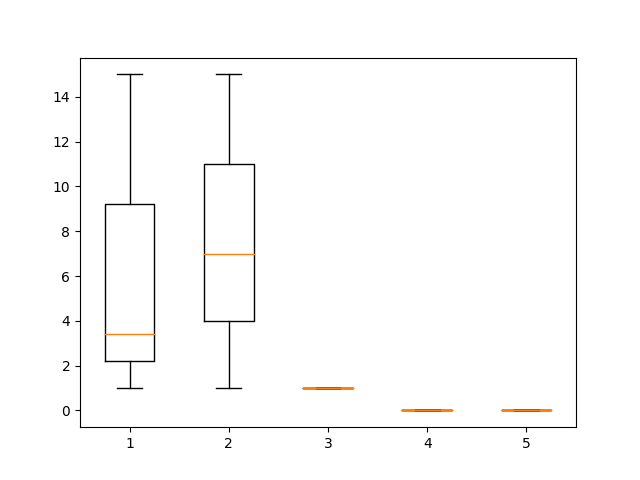
\includegraphics[scale=.5]{16_pasos.png} 
      \caption{16 pasos caja bigote} 
      \label{cam16}
    \end{figure}

    \begin{figure}[H]
      \centering                      % centra la imagen 
      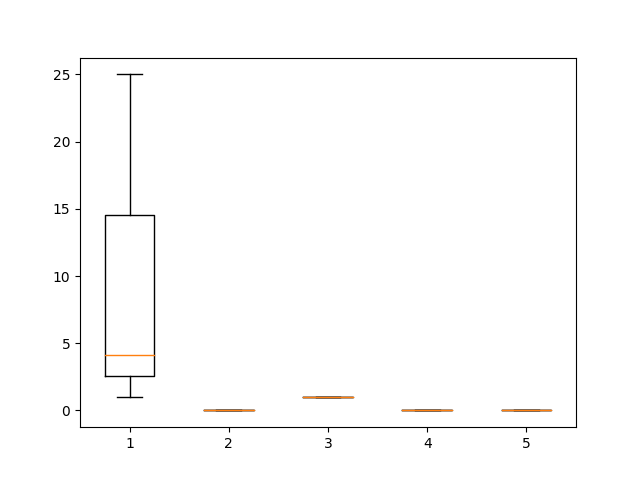
\includegraphics[scale=.5]{32_pasos.png} 
      \caption{32 pasos caja bigote} 
      \label{cam32}
    \end{figure}

    \begin{figure}[H]
      \centering                      % centra la imagen 
      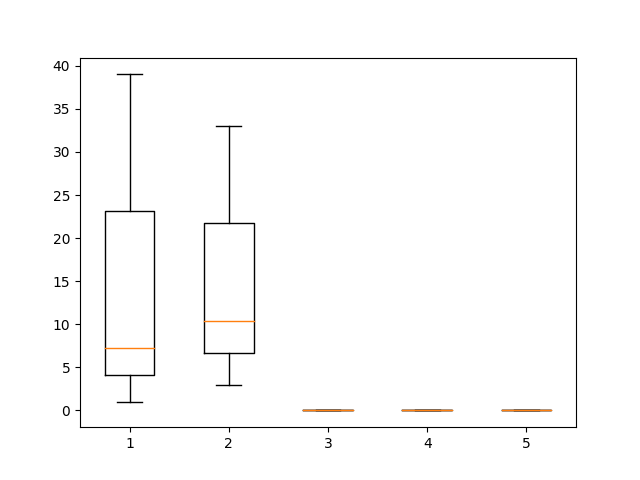
\includegraphics[scale=.5]{64_pasos.png}  
      \caption{64 pasos caja bigote} 
      \label{cam64}
    \end{figure}

    \begin{figure}[H]
      \centering                      % centra la imagen 
      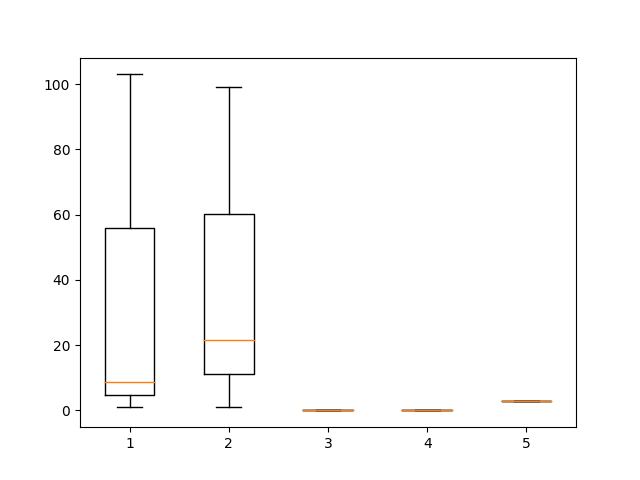
\includegraphics[scale=.5]{128_pasos.png} 
      \caption{128 pasos caja bigote} 
      \label{cam128}
    \end{figure}

    \begin{figure}[H]
      \centering                      % centra la imagen 
      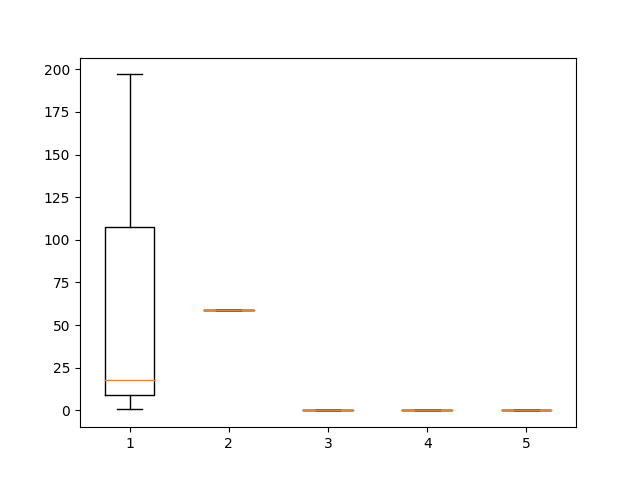
\includegraphics[scale=.5]{256_pasos.png}   
      \caption{256 pasos caja bigote} 
      \label{cam256}
    \end{figure}

    \begin{figure}[H]
      \centering                      % centra la imagen 
      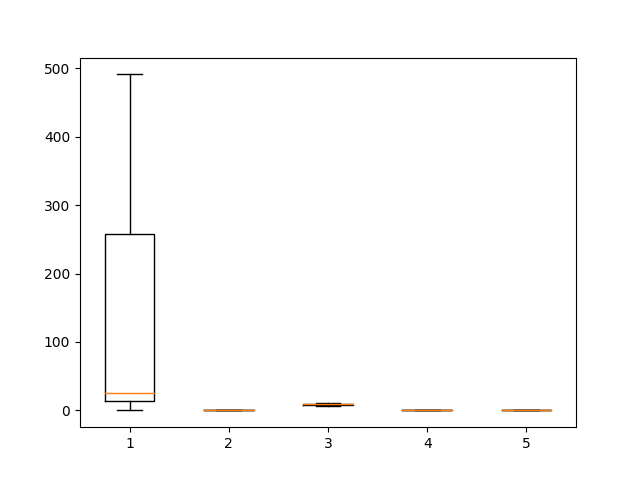
\includegraphics[scale=.5]{512_pasos.png}   
      \caption{512 pasos caja bigote} 
      \label{cam512}
    \end{figure}
observamos una tendencia a desaparecer conforme aumentan las dimensiones, ya casi no regresa a origen nuestro numero al azar debido a que es menos probable que coincidan los orígenes conforme aumenta la dimensión.Solo en dimensiones 1 y 2 se logra ver que se mantienen los regresos constantes como se puede ver en la figura \ref{cam16} y la figura \ref{cam64}.

A continuación se muestran las tablas en donde se obtuvieron datos por dimensión tanto el mínimo de regresos al origen , el máximo , el promedio de estos así como el porcentaje de los que no regresaron, esto para de igual manera 16,32,64,128,256 y 512 pasos y en base a estos llegar a las mismas conclusiones que en las gráficas caja bigote.
    \begin{figure}[H]
      \centering                      % centra la imagen 
      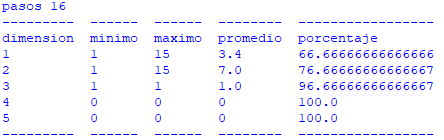
\includegraphics[scale=1.1]{16_pasos_tabla.png} 
      \caption{16 pasos tabla} 
      \label{tab16}
    \end{figure}

    \begin{figure}[H]
      \centering                      % centra la imagen 
      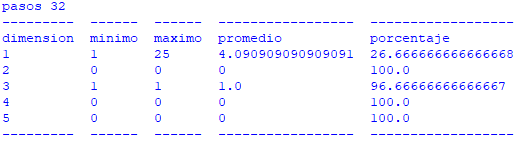
\includegraphics[scale=1]{32_pasos_tabla.png} 
      \caption{32 pasos tabla} 
      \label{tab32}
    \end{figure}

    \begin{figure}[H]
      \centering                      % centra la imagen 
      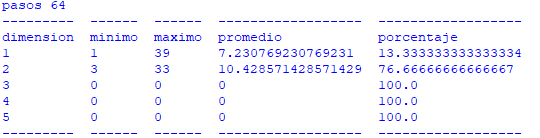
\includegraphics[scale=1]{64_pasos_tabla.png}  
      \caption{64 pasos tabla} 
      \label{tab64}
    \end{figure}

    \begin{figure}[H]
      \centering                      % centra la imagen 
      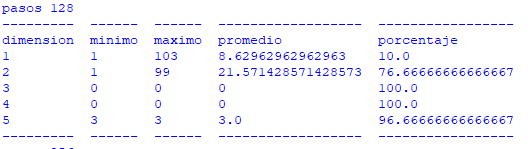
\includegraphics[scale=1]{128_pasos_tablas.png} 
      \caption{128 pasos tabla} 
      \label{tab128}
    \end{figure}

    \begin{figure}[H]
      \centering                      % centra la imagen 
      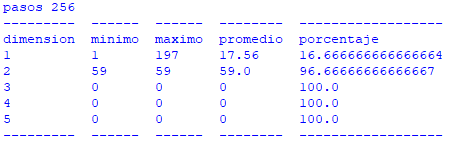
\includegraphics[scale=1.1]{256_pasos_tabla.png}   
      \caption{256 pasos tabla} 
      \label{tab256}
    \end{figure}

    \begin{figure}[H]
      \centering                      % centra la imagen 
      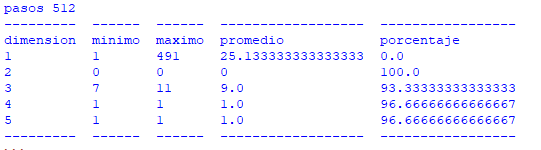
\includegraphics[scale=1]{512_pasos_tabla.png}   
      \caption{512 pasos tabla} 
      \label{tab512}
    \end{figure}
\section{referencias}


    \bibliography{bibliografia.bib}
    [1]Elisa scaeffer. Practica 1,Feb. 2021,https://elisa.dyndns-web.com/teaching/comp/par/p1.html
    
    [2]Python Software Foundation:Guido van Rossum ,2021,https://www.python.org/
    
    [3]Entrenamiento python basico:covantec,2021,https://entrenamiento-python-basico.readthedocs.io/es/latest/


\end{document}